\chapter{Results and Discussion}

Scores are from the official validation splits, and WEMoE rows give the mean and sample standard deviation over seeds 0, 1 and 2. Values come from the first full run of the project (Section~\ref{sec:limitations}).

\section{Performance Evaluation}

Table~\ref{tab:main} and Figure~\ref{fig:per-task} present the main comparison. Task Arithmetic reaches an average of 57.4, moderately above the majority floor of 45.8, and router initialisation alone does not change this ($57.8\pm0.6$). Training the routers with FSFT at $k=256$ raises the full-MLP model to $69.9\pm0.1$, which is 12.5 points above Task Arithmetic and 8.3 below the experts.

\begin{table}[htbp]
  \centering\tablestyle
  \caption{Validation scores ($\times100$). Task Arithmetic uses $\lambda=0.3$; FSFT and router-init rows are WEMoE with $k=256$. Bold marks the best merged model in each column.}
  \label{tab:main}
  \setlength{\tabcolsep}{3pt}\begin{tabularx}{\linewidth}{X c c c c c c c r r}
    \toprule
    Model & MRPC acc & MRPC F1 & RTE & CoLA & SST-2 & QNLI & Avg & Norm. & Gain\\
    \midrule
    Majority class & 68.4 & 81.2 & 52.7 & 0.0 & 50.9 & 50.5 & 45.8 & 56.4 & 0.0\\
    Simple Averaging & 68.4 & 81.2 & 46.9 & 23.3 & 55.4 & 65.9 & 53.3 & 66.8 & 6.6\\
    Task Arithmetic & 68.6 & 81.3 & 47.3 & 16.9 & 69.8 & 77.9 & 57.4 & 70.6 & 18.4\\
    Router init, full & 68.5$\pm$0.1 & 81.3$\pm$0.1 & 47.1$\pm$0.2 & 19.3$\pm$2.0 & 70.2$\pm$1.1 & 77.7$\pm$0.2 & 57.8$\pm$0.6 & 71.3 & 18.7\\
    FSFT, full MLP & \textbf{76.3}$\pm$4.5 & \textbf{83.9}$\pm$2.8 & 52.0$\pm$4.4 & \textbf{42.6}$\pm$0.9 & \textbf{88.0}$\pm$0.5 & \textbf{86.7}$\pm$0.7 & \textbf{69.9}$\pm$0.1 & \textbf{87.8} & \textbf{59.1}\\
    FSFT, intermediate & 66.5$\pm$0.7 & 76.6$\pm$1.0 & \textbf{59.0}$\pm$0.9 & 41.7$\pm$0.9 & 86.7$\pm$0.2 & 86.5$\pm$0.2 & 69.1$\pm$0.1 & 87.4 & 54.8\\
    \midrule
    Experts & 82.1 & 88.1 & 63.2 & 59.1 & 92.2 & 91.2 & 78.2 & 100.0 & 100.0\\
    \bottomrule
  \end{tabularx}
\end{table}

\begin{figure}[htbp]
  \centering
  % Palette: reference categorical order validated with the dataviz validator (contrast WARN is relieved by the
% marker shapes, the legend and Table~\ref{tab:main}).
\definecolor{sA}{HTML}{2A78D6}\definecolor{sB}{HTML}{EB6834}\definecolor{sC}{HTML}{1BAF7A}
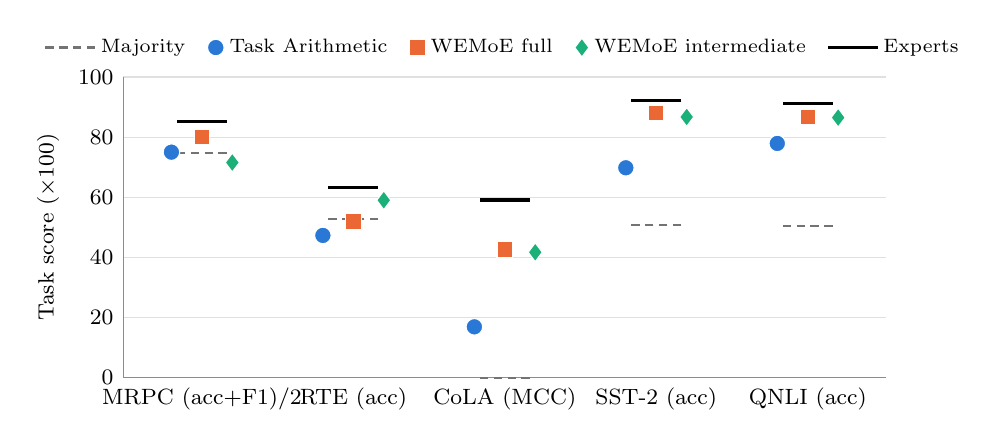
\begin{tikzpicture}
\begin{axis}[
  width=.93\linewidth, height=5.4cm,
  symbolic x coords={MRPC,RTE,CoLA,SST-2,QNLI}, xtick=data, enlarge x limits=.13,
  xticklabels={{MRPC (acc+F1)/2},{RTE (acc)},{CoLA (MCC)},{SST-2 (acc)},{QNLI (acc)}},
  ymin=0, ymax=100, ytick={0,20,40,60,80,100}, ylabel={Task score ($\times100$)},
  ymajorgrids, grid style={black!12}, axis line style={black!45}, tick style={draw=none},
  tick label style={font=\footnotesize}, label style={font=\footnotesize},
  clip=false, axis x line*=bottom, axis y line*=left,
  legend style={at={(.5,1.03)},anchor=south,legend columns=5,draw=none,font=\scriptsize,/tikz/every even column/.append style={column sep=6pt}},
]
\addplot[only marks,mark=-,mark size=9pt,thick,black!55,densely dashed] coordinates {(MRPC,74.8) (RTE,52.7) (CoLA,0) (SST-2,50.9) (QNLI,50.5)};
\addlegendentry{Majority}
\addplot[only marks,mark=*,mark size=3pt,sA,mark options={fill=sA,draw=white},xshift=-11pt] coordinates {(MRPC,75.0) (RTE,47.3) (CoLA,16.9) (SST-2,69.8) (QNLI,77.9)};
\addlegendentry{Task Arithmetic}
\addplot[only marks,mark=square*,mark size=2.8pt,sB,mark options={fill=sB,draw=white}] coordinates {(MRPC,80.1) (RTE,52.0) (CoLA,42.6) (SST-2,88.0) (QNLI,86.7)};
\addlegendentry{WEMoE full}
\addplot[only marks,mark=diamond*,mark size=3.4pt,sC,mark options={fill=sC,draw=white},xshift=11pt] coordinates {(MRPC,71.55) (RTE,59.0) (CoLA,41.7) (SST-2,86.7) (QNLI,86.5)};
\addlegendentry{WEMoE intermediate}
\addplot[only marks,mark=-,mark size=9pt,very thick,black] coordinates {(MRPC,85.1) (RTE,63.2) (CoLA,59.1) (SST-2,92.2) (QNLI,91.2)};
\addlegendentry{Experts}
\end{axis}
\end{tikzpicture}

  \caption{Task scores of the merged models between the majority floor (dashed tick) and the experts (solid tick). WEMoE values use $k=256$ and are means over three seeds; Table~\ref{tab:main} gives standard deviations.}
  \label{fig:per-task}
\end{figure}

The normalised score suggests that Task Arithmetic retains 70.6\% of expert performance, but the gain reveals that it captures only 18.4\% of the distance between a constant guess and the expert, compared with 59.1\% for WEMoE + FSFT. Task Arithmetic's accuracy on RTE (47.3) equals 131/277, the share of the \emph{minority} class, which indicates a constant prediction.

\section{Comparison with Individual Experts}

Table~\ref{tab:gain} shows each merged model's position per task. On SST-2 and QNLI the trained routers recover close to 90\% of the available gain, and on CoLA about 70\%. MRPC and RTE, the two smallest tasks, depend on the upscaling scope: the full-MLP model recovers about half of the gain on MRPC but stays marginally below the majority on RTE, whereas the intermediate-only model recovers 60\% on RTE but falls below the majority on MRPC. No merged model matches an expert on any task.

\begin{table}[htbp]
  \centering\tablestyle
  \caption{Gain over majority per task, in percent, computed from the seed means. Zero is a constant guess and 100 is the expert.}
  \label{tab:gain}
  \begin{tabular}{l r r r r r r}
    \toprule
    Model & MRPC & RTE & CoLA & SST-2 & QNLI & Mean\\
    \midrule
    Task Arithmetic & 2 & $-52$ & 29 & 46 & 67 & 18.4\\
    WEMoE + FSFT, full MLP, $k=256$ & 51 & $-7$ & 72 & 90 & 89 & 59.1\\
    WEMoE + FSFT, intermediate-only, $k=256$ & $-32$ & 60 & 71 & 87 & 88 & 54.8\\
    \bottomrule
  \end{tabular}
\end{table}

The labelled budget strongly influences results (Table~\ref{tab:budget}). The average grows with $k$, but stability is the more informative finding: the standard deviation of CoLA's MCC is 14.1 and 17.8 at $k=16$ and $k=64$ (individual runs span 18--44 and 9--41), and 0.9 at $k=256$. Small budgets also reach their best development score early, consistent with overfitting: 7.1M router parameters face only 80 to 320 training examples.

\begin{table}[htbp]
  \centering\tablestyle
  \caption{Effect of the labelled budget on the full-MLP model. Best steps are listed per seed; n/a marks those not retained.}
  \label{tab:budget}
  \setlength{\tabcolsep}{3pt}\begin{tabular}{r c c c c c r r r l}
    \toprule
    $k$ & MRPC acc & RTE & CoLA & SST-2 & QNLI & Avg & Norm. & Gain & Best step\\
    \midrule
    16 & 68.7$\pm$2.3 & 48.0$\pm$1.0 & 27.6$\pm$14.1 & 79.6$\pm$8.1 & 74.0$\pm$6.5 & 60.8$\pm$2.7 & 75.6 & 25.5 & 50, n/a, 150\\
    64 & 71.6$\pm$4.4 & 54.0$\pm$3.4 & 20.5$\pm$17.8 & 89.0$\pm$0.6 & 83.1$\pm$2.4 & 64.6$\pm$3.7 & 79.5 & 46.7 & 100, 250, 100\\
    256 & 76.3$\pm$4.5 & 52.0$\pm$4.4 & 42.6$\pm$0.9 & 88.0$\pm$0.5 & 86.7$\pm$0.7 & 69.9$\pm$0.1 & 87.8 & 59.1 & 250, n/a, n/a\\
    \bottomrule
  \end{tabular}
\end{table}

\section{Model Storage and Efficiency}

Table~\ref{tab:storage} reports stored parameters measured on the built models, which match the closed-form counts in the code. Merged models keep one set of non-MLP parameters but retain the pre-trained MLP weights and one task vector per expert for each upscaled module. Task vectors therefore dominate, at 283.3M of the 400.0M parameters of the full-MLP model. This limits the saving over five experts to 26.9\%, whereas intermediate-only upscaling saves 52.8\% and is 35\% smaller than full-MLP.

\begin{table}[htbp]
  \centering\tablestyle
  \caption{Stored floating-point parameters (millions) by component, and total size at 32-bit precision.}
  \label{tab:storage}
  \begin{tabular}{l r r r r r r r r}
    \toprule
    Deployment & Shared & Base MLP & Task vectors & Routers & Heads & Total & GiB & vs.\ 5 models\\
    \midrule
    Five single-task models & -- & -- & -- & -- & -- & 547.4 & 2.04 & 100.0\%\\
    Task Arithmetic & -- & -- & -- & -- & -- & 109.5 & 0.41 & 20.0\%\\
    WEMoE, full MLP & 52.8 & 56.7 & 283.3 & 7.13 & 0.008 & 400.0 & 1.49 & 73.1\%\\
    WEMoE, intermediate-only & 81.1 & 28.3 & 141.7 & 7.13 & 0.008 & 258.4 & 0.96 & 47.2\%\\
    \bottomrule
  \end{tabular}
\end{table}

Because each input here arrives with its task identifier, the five experts could also be selected directly by task, and they are more accurate than full-MLP WEMoE and only 37\% larger. The storage argument therefore rests mainly on the intermediate-only variant, or on scenarios without explicit task identifiers, which this implementation does not evaluate.

\section{Analysis and Discussion}

\begin{figure}[htbp]
  \centering
  \includegraphics[width=.6\linewidth]{routing.png}
  \caption{Mean gating weights per layer and input task (full MLP, $k=256$, seed 0). Blue adds and red subtracts a task vector.}
  \label{fig:routing}
\end{figure}

\paragraph{Learned routing.} Figure~\ref{fig:routing} and the project's run analysis show how far FSFT moves the model from Task Arithmetic. Weights span $-3.0$ to $4.4$, and the per-layer sum reaches 5.8 against 1.5 at initialisation, which a convex mixture could not express. Much of the pattern is shared: mean routing matrices of different input tasks correlate at 0.82 on average, yet the input task still explains about 58\% of the routing variance. Routing is thus partly input-dependent, although this does not show that it causes the gain.

\paragraph{Differences across tasks.} SST-2 and QNLI, where WEMoE does well, have the largest training sets and the strongest experts, whereas MRPC and RTE have the smallest. The RTE failure of the full-MLP model is visible in routing: on RTE inputs the RTE task vector receives an average weight of about 0.01, compared with 1.37 for the MRPC and SST-2 experts on their own inputs, and it is subtracted in layers 11 and 12. With intermediate-only upscaling this weight rises to 0.96 and RTE accuracy to 59.0. A plausible but untested explanation is that objective~\eqref{eq:fsft} and mean-score selection trade tasks against one another, retaining router states whose gains elsewhere outweigh a loss on RTE. The weak RTE expert (63.2) may also supply a less useful task vector.

\paragraph{Sampling noise.} Approximate standard errors of accuracy are 3.0 points on RTE ($n=277$) and 2.1 on MRPC ($n=408$). The 0.8-point gap between scopes and RTE's 52.0 versus the majority's 52.7 are therefore within noise.

\paragraph{Trade-offs.} Task Arithmetic is the smallest deployment but performs poorly. Intermediate-only WEMoE stores less than half of five experts with a similar average to the full-MLP model and about half its router training time (8.5 versus 14--16 minutes per run on the T4); its best step came late (400--500 of 500). Full-MLP WEMoE has the highest gain but approaches the size of the experts.

\paragraph{Relation to the original study.} Tang et al.\ report that WEMoE approaches individual fine-tuned models on image tasks, whereas a clear gap remains here, but tasks, backbone, objective and data all differ.

\section{Limitations}
\label{sec:limitations}

First, ``few-shot'' is not strict in the sense of Perez et al.~\cite{perez2021truefewshot}: the best step is selected on up to 1,000 labelled examples per task, against $k=256$ for FSFT. Second, standard deviations exclude expert and data-split variation. Third, per-run outputs were only partly retained: seven of the twelve FSFT runs keep their raw results, and per-example predictions were not retained, so routing statistics come from the project's written run analysis. Results for the input-independent router are unavailable.